%
% NOS
%
% Aleph Objects Firewall
%
% Copyright (C) 2014, 2015, 2016 Aleph Objects, Inc.
%
% This document is licensed under the Creative Commons Attribution 4.0
% International Public License (CC BY-SA 4.0) by Aleph Objects, Inc.
%
There are a lot of operating systems to consider to use as a firewall...

\section{Requirements}

Notes on some requirements in a firewall.

\begin{itemize}
 \item Must be free software.
 \item The project must still be alive.
 \item Does it use a hardened kernel?
 \item How does it do security updates?
 \item Are there open security issues?
 \item Are there any CVEs?
 \item How are security issues handled?
 \item Is there a list of security issues?
 \item Does it have a wifi portal? (Should that be a separate box or in OpenWRT?)
 \item Does upstream https actually work?
 \item UTM - Unified Threat Management (e.g. snort, etc.)
 \item Load balancing between multiple upstreams (without BGP).
 \item Load balancing between dual local routers.
 \item Fail over to standby router (e.g. pfsync).
 \item ``Anti-virus'', SMTP, POP scans? Meh? (e.g. OpenBSD has greylist/tarpit.)
 \item Packet cleansing (e.g. tcp header randomization).
 \item Do we want DNS, DHCP, etc? Probably not?
 \item OpenVPN (built into router, or thru it?).
 \item Network graphing (MRTG, aguri, etc.)
 \item No broken ``community'' editions.
 \item Have mirrored server doing analysis?
 \item NAT options? cone, etc.
 \item Local system monitoring (e.g. system temp, hdd status, etc.)
 \item sshd
 \item GSM, pppd ?
 \item Two-factor authentication.
 \item snort, suricata
\end{itemize}


\section{Firewall Operating Systems in Use}
\subsection{Debian}
 \href{https://www.debian.org/}{Debian}

Aleph Objects uses Debian for nearly everything. It could easily be used as a
router/firewall. There are better, more tuned options.

Linux's iptables is used on servers.

\begin{figure}[h!]
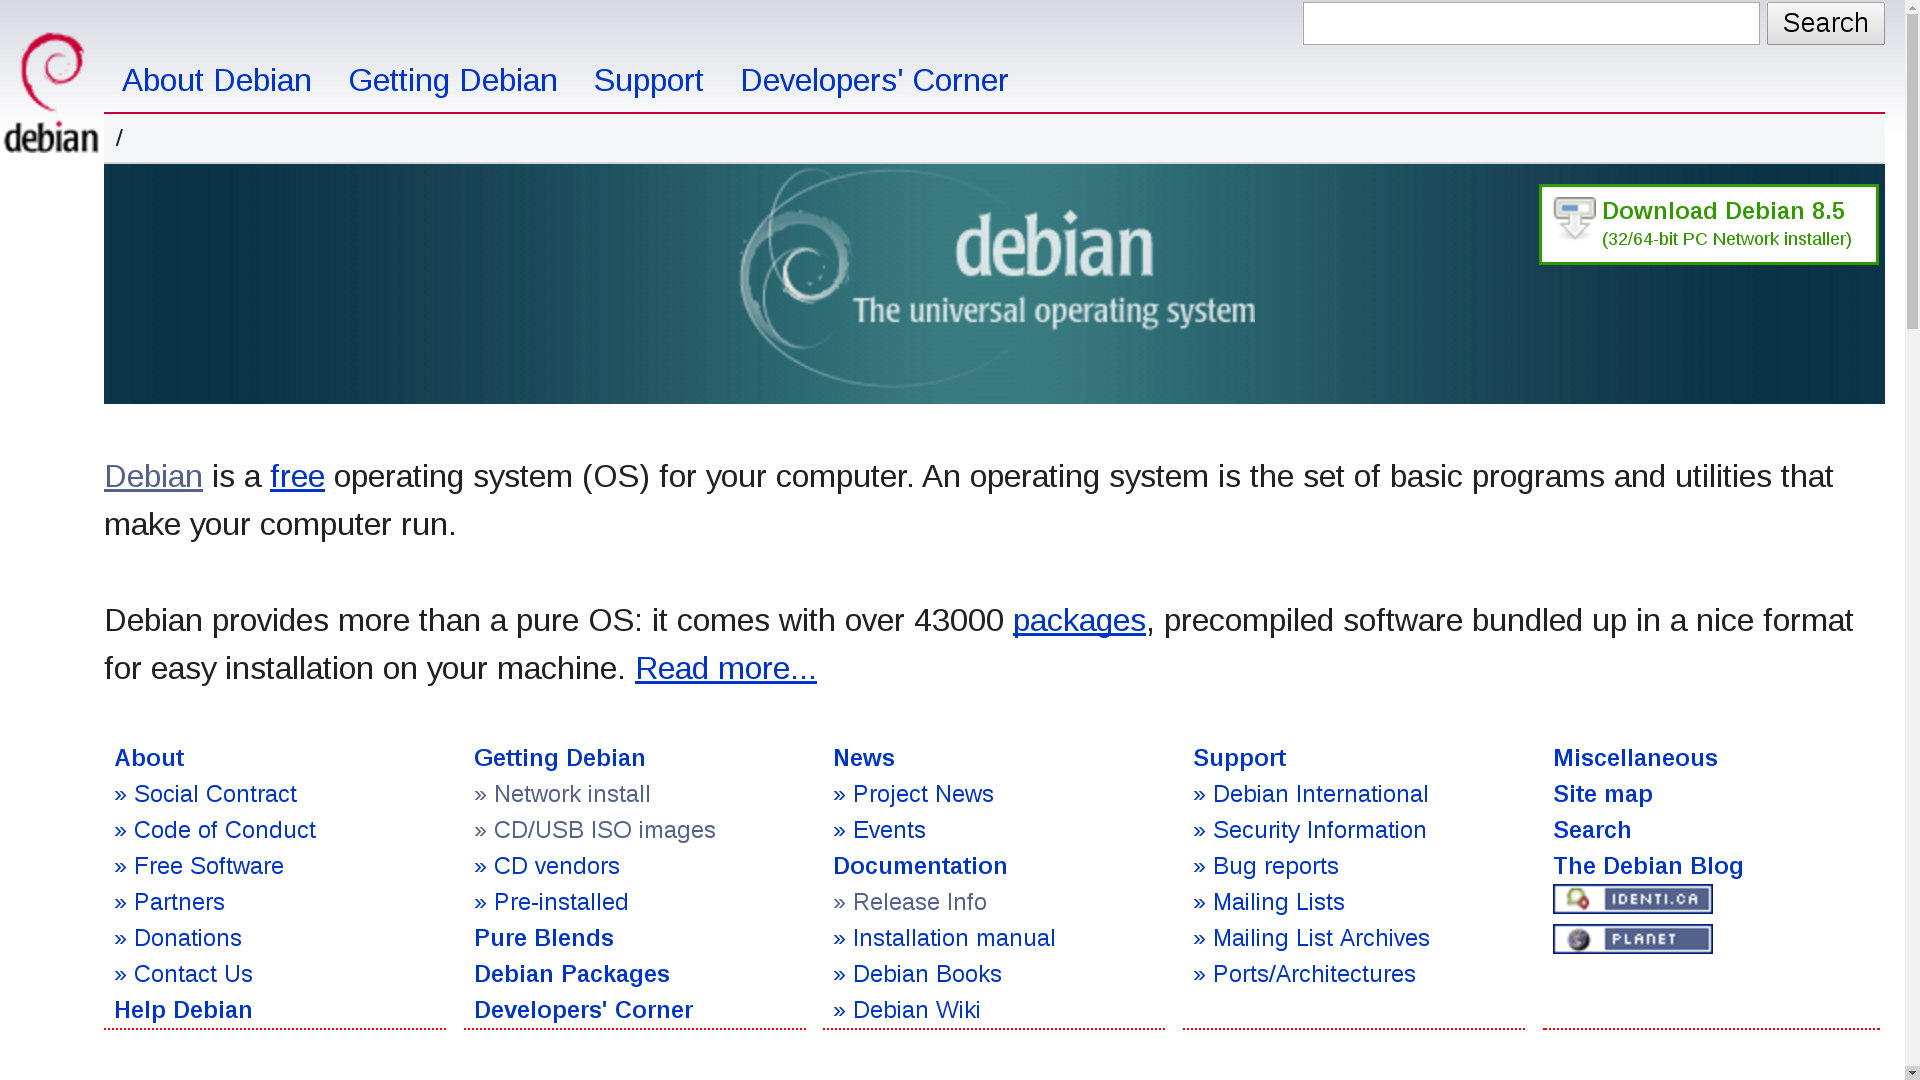
\includegraphics[keepaspectratio=true,height=1.10\textheight,width=1.00\textwidth,angle=0]{www-debian.png}
 \caption{Debian Website}
 \label{fig:www-debian}
\end{figure}


\subsection{pfSense}
\href{https://www.pfsense.org/}{pfSense}

pfSense is used for the main firewalls. See pfSense chapter for more info.


\subsection{FreeBSD}
 \href{https://www.freebsd.org/}{FreeBSD}

FreeBSD is used as the base for pfSense.

\begin{figure}[h!]
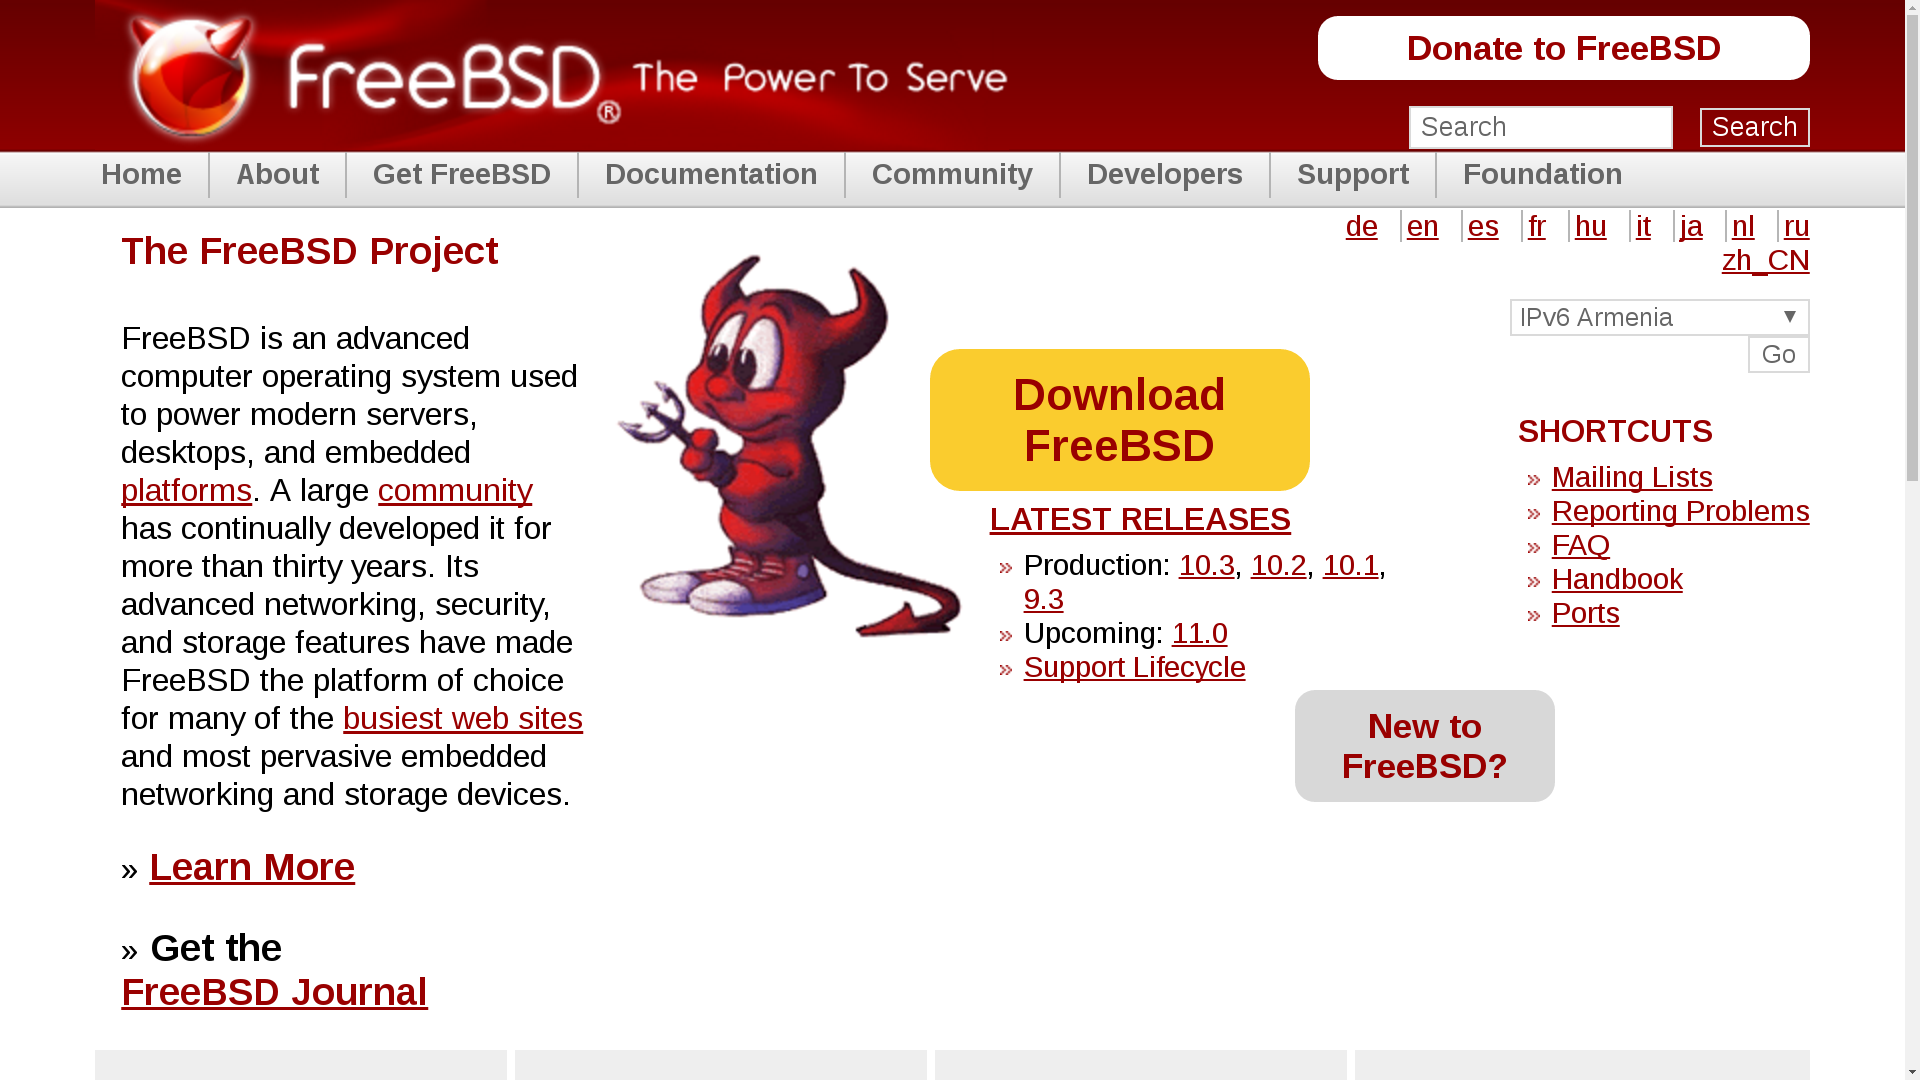
\includegraphics[keepaspectratio=true,height=1.10\textheight,width=1.00\textwidth,angle=0]{www-freebsd.png}
 \caption{FreeBSD Website}
 \label{fig:www-freebsd}
\end{figure}

Solid OS. Can use OpenBSD's PF (packet filtering). Same problem as with
OpenBSD, few admins know it.


\section{Firewalls Evaluated}
The following firewalls were installed and tested for evaluation. pfSense was
selected over these due to it being Free Software, its high security, the vast
feature set, regular maintenance, and just being glorious overall.

\subsection{pfSense}

A few notes from the initial pfSense test install:

\begin{itemize}
 \item Released May 18th, 2016.
 \item pfSense-CE-memstick-2.3.1-RELEASE-amd64.img
 \item FreeBSD 10.3 based.
 \item Installer feels like a step back in computing history.
 \item First boot goes to console with lots of useful options.
 \item Web admin wizard mentions pfSense Gold Subscriptions. It doesn't appear to be for non-free software (e.g. isn't baitware).
 \item They sell very nice looking hardware with pfsense pre-installed. With failover systems (CARP).
 \item Load balancing, failover.
 \item Clean and very responsive web interface (based on Bootstrap).
 \item Web based updater to new minor version.
 \item x86 architecture only.
 \item Looks to have good security errata process, following FreeBSD.
 \item Snort threat lists are available. Paid for more recent ones, same as on other snort platforms.
 \item Installation of additional packages is clean, and doesn't appear to offer any non-free.
 \item ClamAV ...
\end{itemize}


\subsection{Alpine Linux}
 \href{https://www.alpinelinux.org/}{Alpine} --- ``Small. Simple. Secure. Alpine Linux is a security-oriented, lightweight Linux distribution based on musl libc and busybox.''

\begin{figure}[h!]
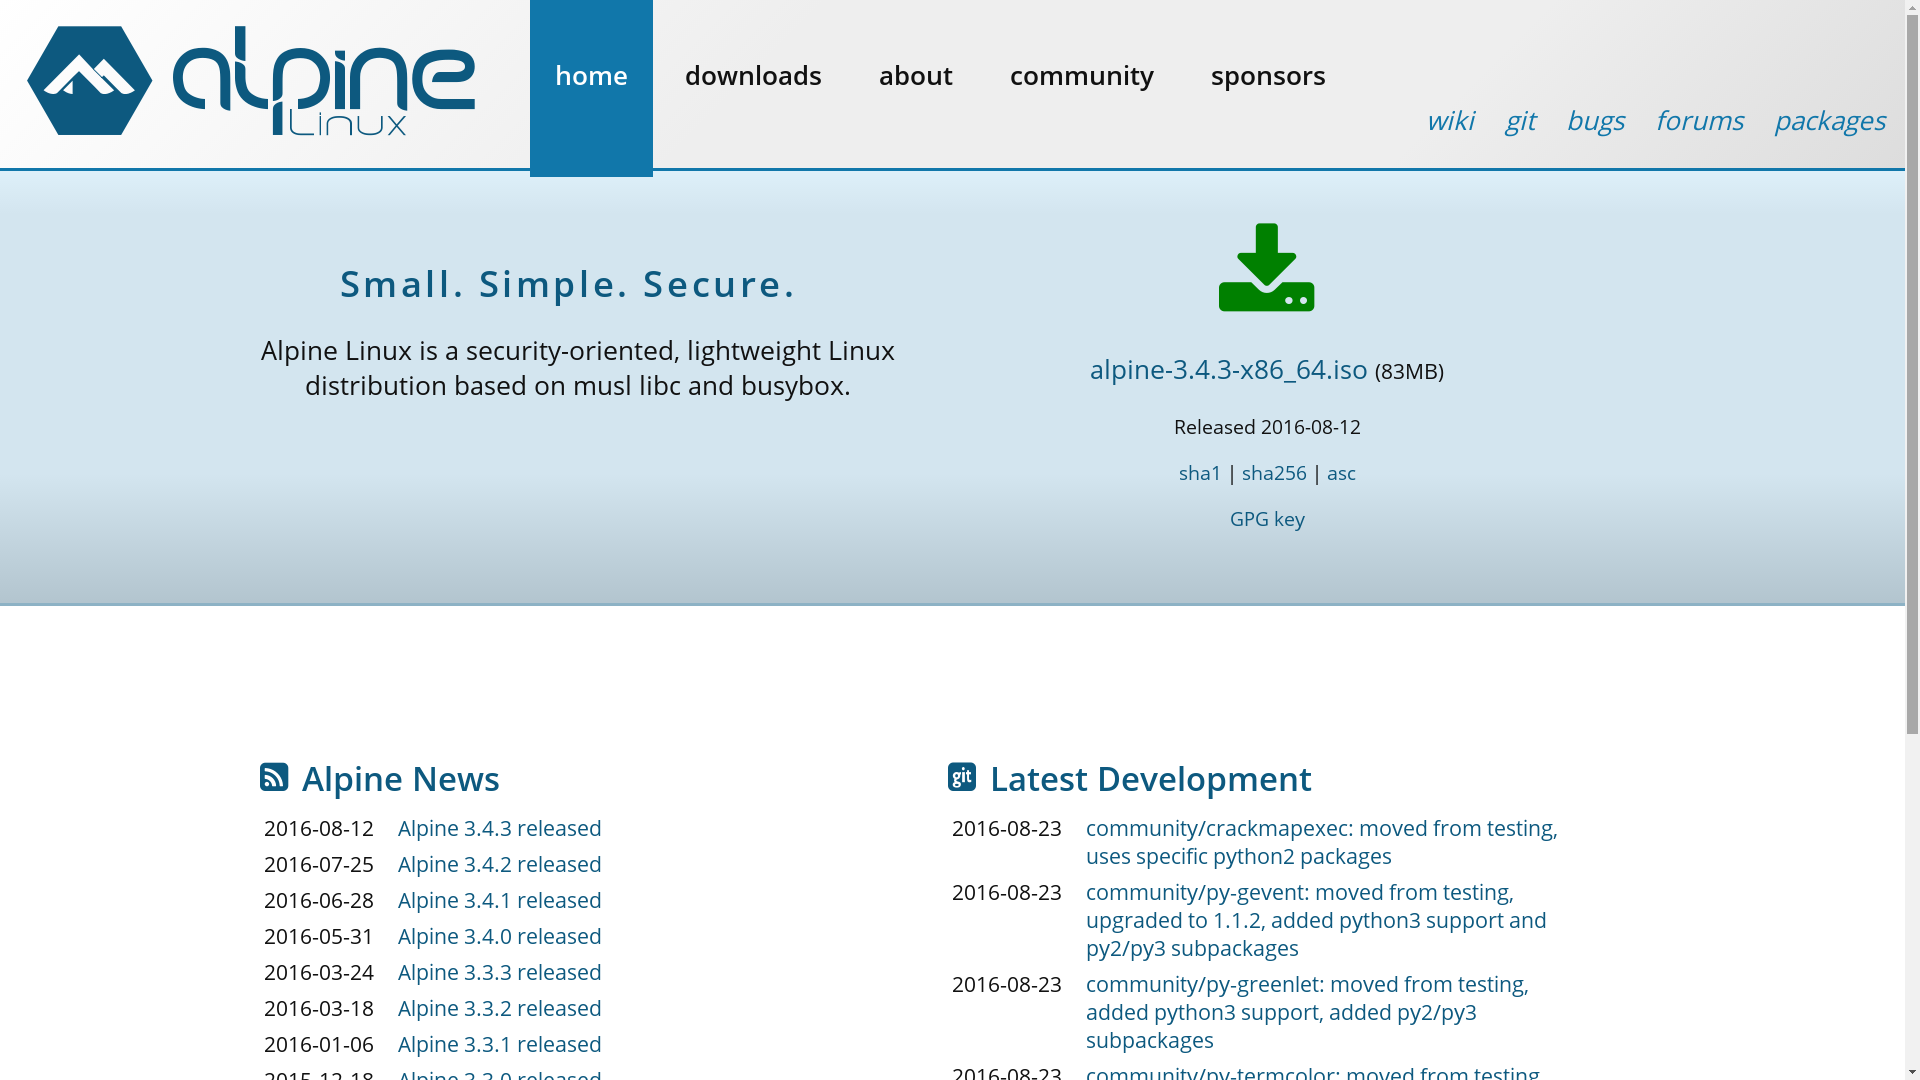
\includegraphics[keepaspectratio=true,height=1.10\textheight,width=1.00\textwidth,angle=0]{www-alpine.png}
 \caption{Alpine Linux Website}
 \label{fig:www-alpine}
\end{figure}

Download and install .iso to USB. Boot from USB, do text install onto HD. The installer looked very much like OpenBSD and was quite terse, but worked fine.
The installed system is a basic lean GNU/Linux installation. Firewall configuration is text based. Looks nice, but not many features, except lightweight.
Similar to OpenWRT in that way, except no web GUI, AFAICT.


\subsection{clearOS}

\href{https://www.clearos.com/}{clearOS} --- ``ClearOS is an operating system for your Server, Network, and Gateway systems. It is designed for homes, small to medium businesses, and distributed environments. ClearOS is commonly known as the Next Generation Small Business Server, while including indispensable Gateway and Networking functionality. It delivers a powerful IT solution with an elegant user interface that is completely web-based.''

\begin{figure}[h!]
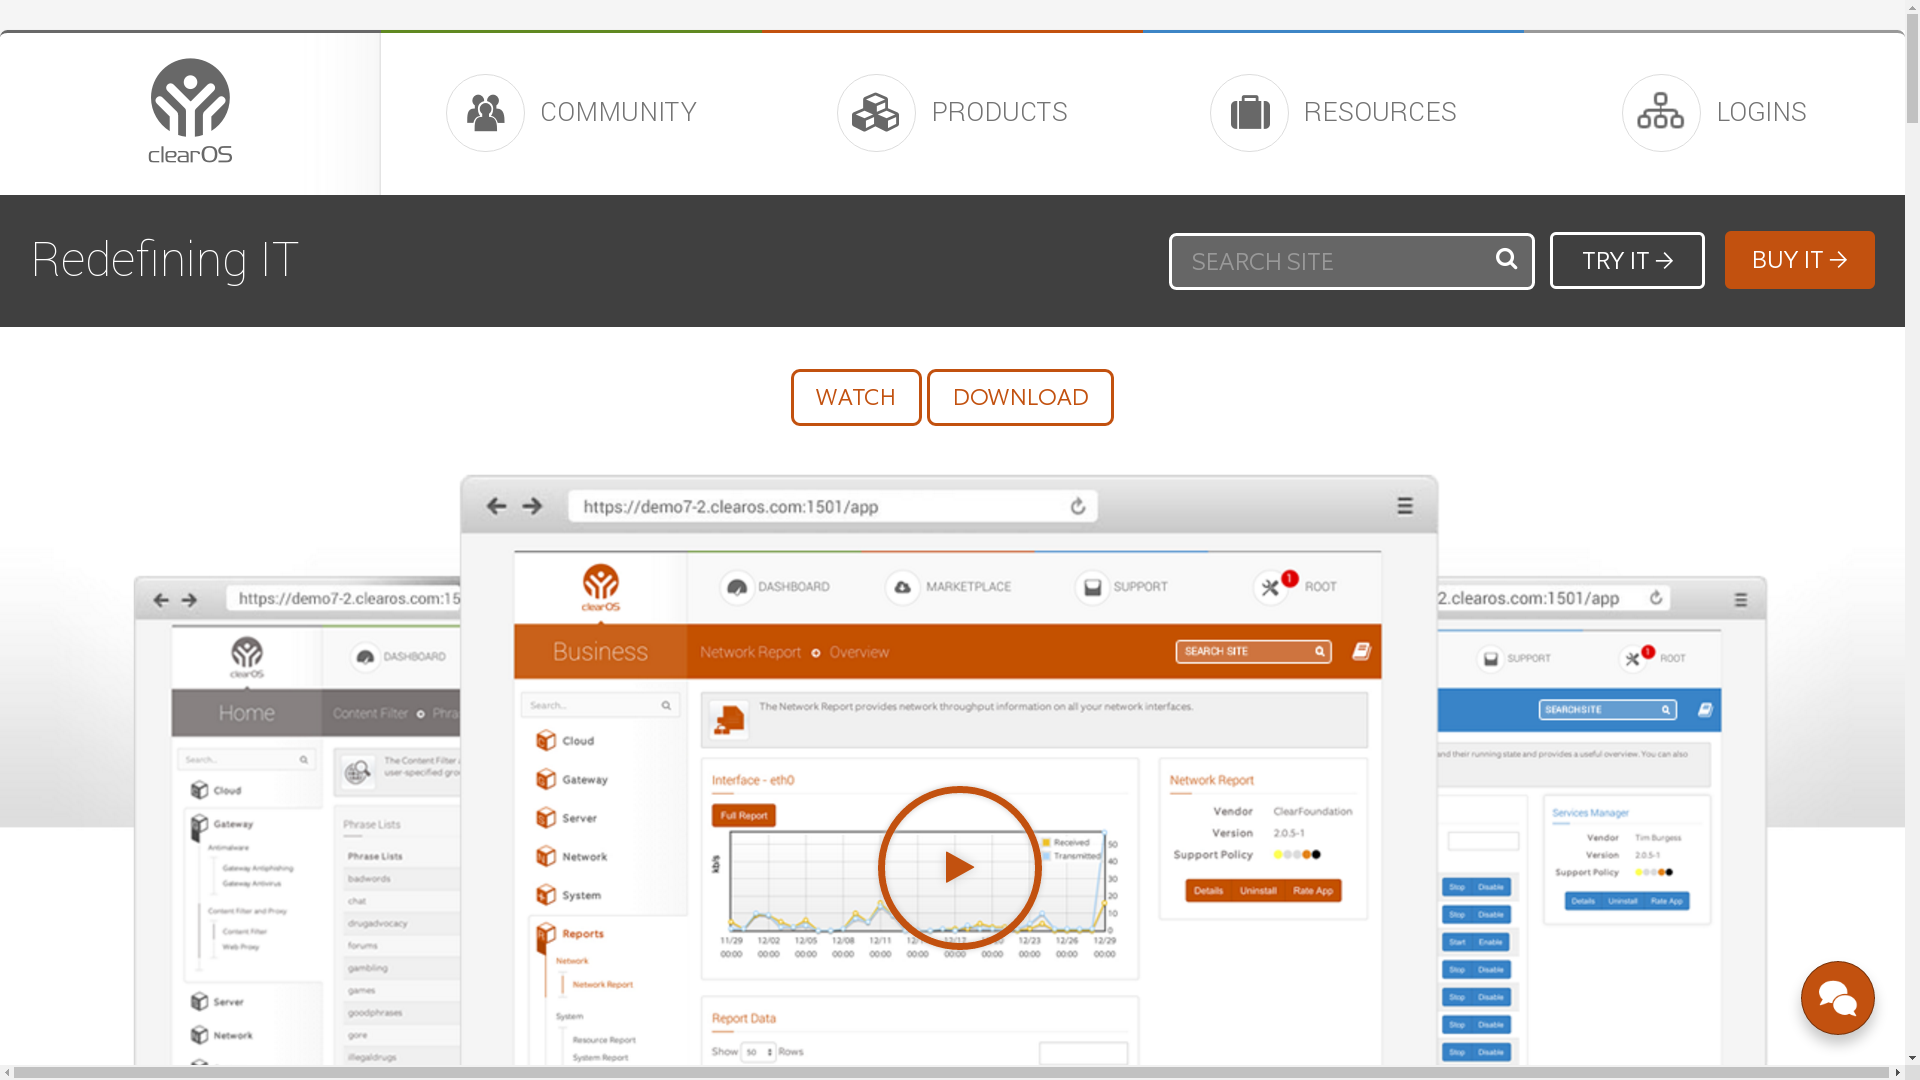
\includegraphics[keepaspectratio=true,height=1.10\textheight,width=1.00\textwidth,angle=0]{www-clearos.png}
 \caption{clearOS Website}
 \label{fig:www-clearos}
\end{figure}

\begin{itemize}
 \item Overall, very very nice, very clean with many features.
 \item Baitware is the only thing holding this back.
 \item The web interface never crashed or caused issues.
 \item Usage is stable.
 \item Latest release: 7.2.0
 \item Release Date: March 7, 2015.
 \item Package Updater: yum
 \item Kernel: Linux 3.10.0-327.3.1.el17.x86\_64
 \item Base OS: Fedora? CentOS?
 \item Easy GUI install
 \item Has enterprise (baitware?) version.
 \item Has enterprise hardware.
 \item Web based configuration system started on first boot
 \item Web wizard has option to select Community or non-free versions.
 \item Web wizard has system registration for a marketplace for apps. Have to register?
 \item Registering set ``Software End-of-Life'' to August 31, 2018.
 \item Lots of phone-home activity with marketplace and registration....
 \item Simple ``Update All'' button to update system (with yum, afaict).
 \item Very clean, overall.
 \item Wide variety of ``Apps'' in the Marketplace that are GPL.
 \item Non-free plugins are listed along free ones. The owncloud plugin is non-free.
 \item Most apps don't have any ratings.
 \item The default ``Exception Sites'' whitelist had their clear*.com sites and a few *.microsoft.com.
 \item Has optionally transparent web proxy.
 \item Installed many Apps, and it was all very clean.
 \item clearOS gets pwned, we get pwnd? Yes.
 \item Need to create account to get to knowledge base ?
 \item Actual firewalling rules (e.g. block just these devices from everything but port 443) aren't so strong.
 \item There doesn't appear to be a way to say ``just allow port 22 from NNN''...
 \item A lot of great setup.
 \item MultiWAN --- Nice, but simple load balancing between multiple upstreams.
 \item Failover to multiple upstreams.
 \item No fail over to another router (ala CARP).
 \item dhclient (?) overwrites DNS addresses, no place to set static (?!?)
 \item Some pretty graphs, but not the most useful.
 \item Overall kind of a toy compared to pfSense.
\end{itemize}


\subsection{IPCop}
\href{http://www.ipcop.org/}{IPCop} --- ``The IPCop Firewall is a Linux firewall distribution. It is geared towards home and SOHO users. The IPCop web-interface is very user-friendly and makes usage easy.''

\begin{figure}[h!]
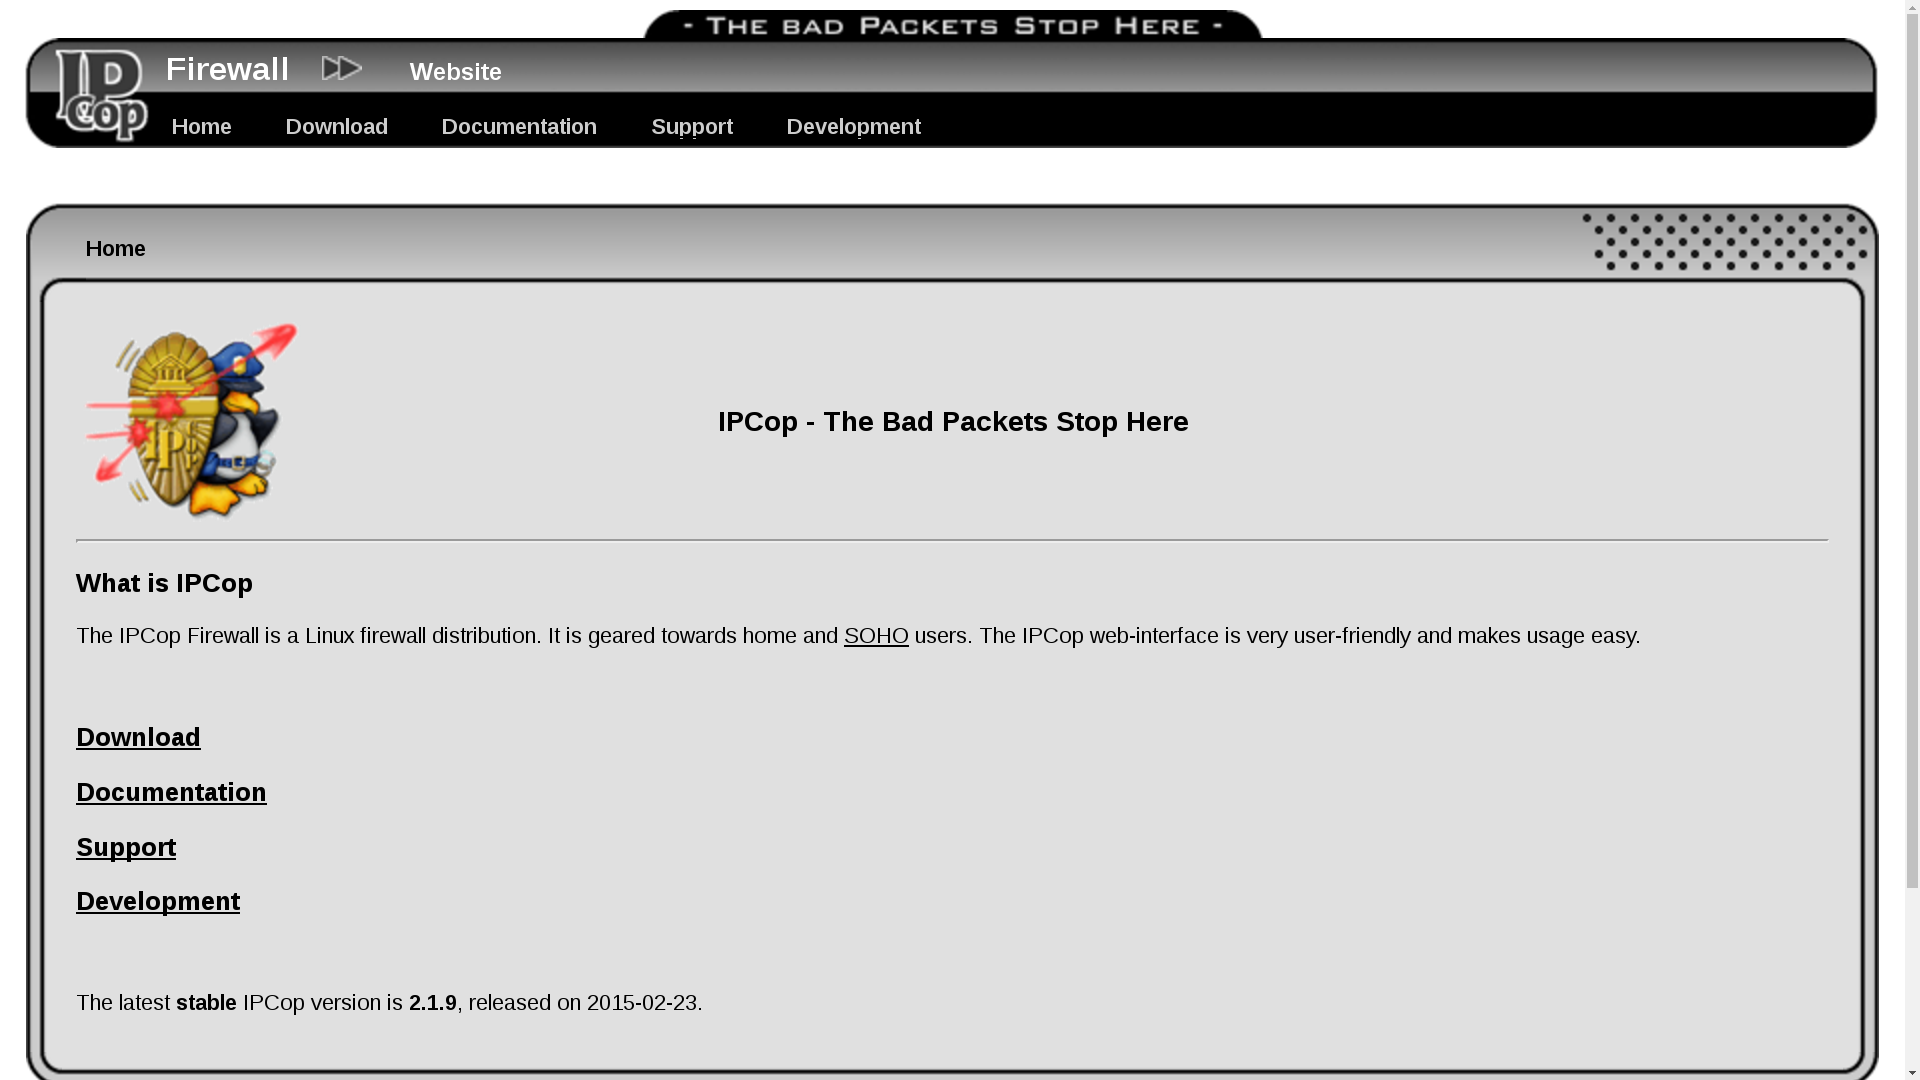
\includegraphics[keepaspectratio=true,height=1.10\textheight,width=1.00\textwidth,angle=0]{www-ipcop.png}
 \caption{IPCop Website}
 \label{fig:www-ipcop}
\end{figure}


\begin{itemize}
 \item Last release was 2015-02-23, well over a year ago.
 \item The i486 image doesn't boot all the way, gives video artifacts.
 \item All looks pretty old and crufty at this point.
\end{itemize}


\subsection{IPFire}
\href{http://www.ipfire.org/}{IPFire} --- ``the professional and hardened Linux firewall distribution that is secure, easy to operate and coming with great functionality so that it is ready for enterprises, authorities, and anybody else.''

\begin{figure}[h!]
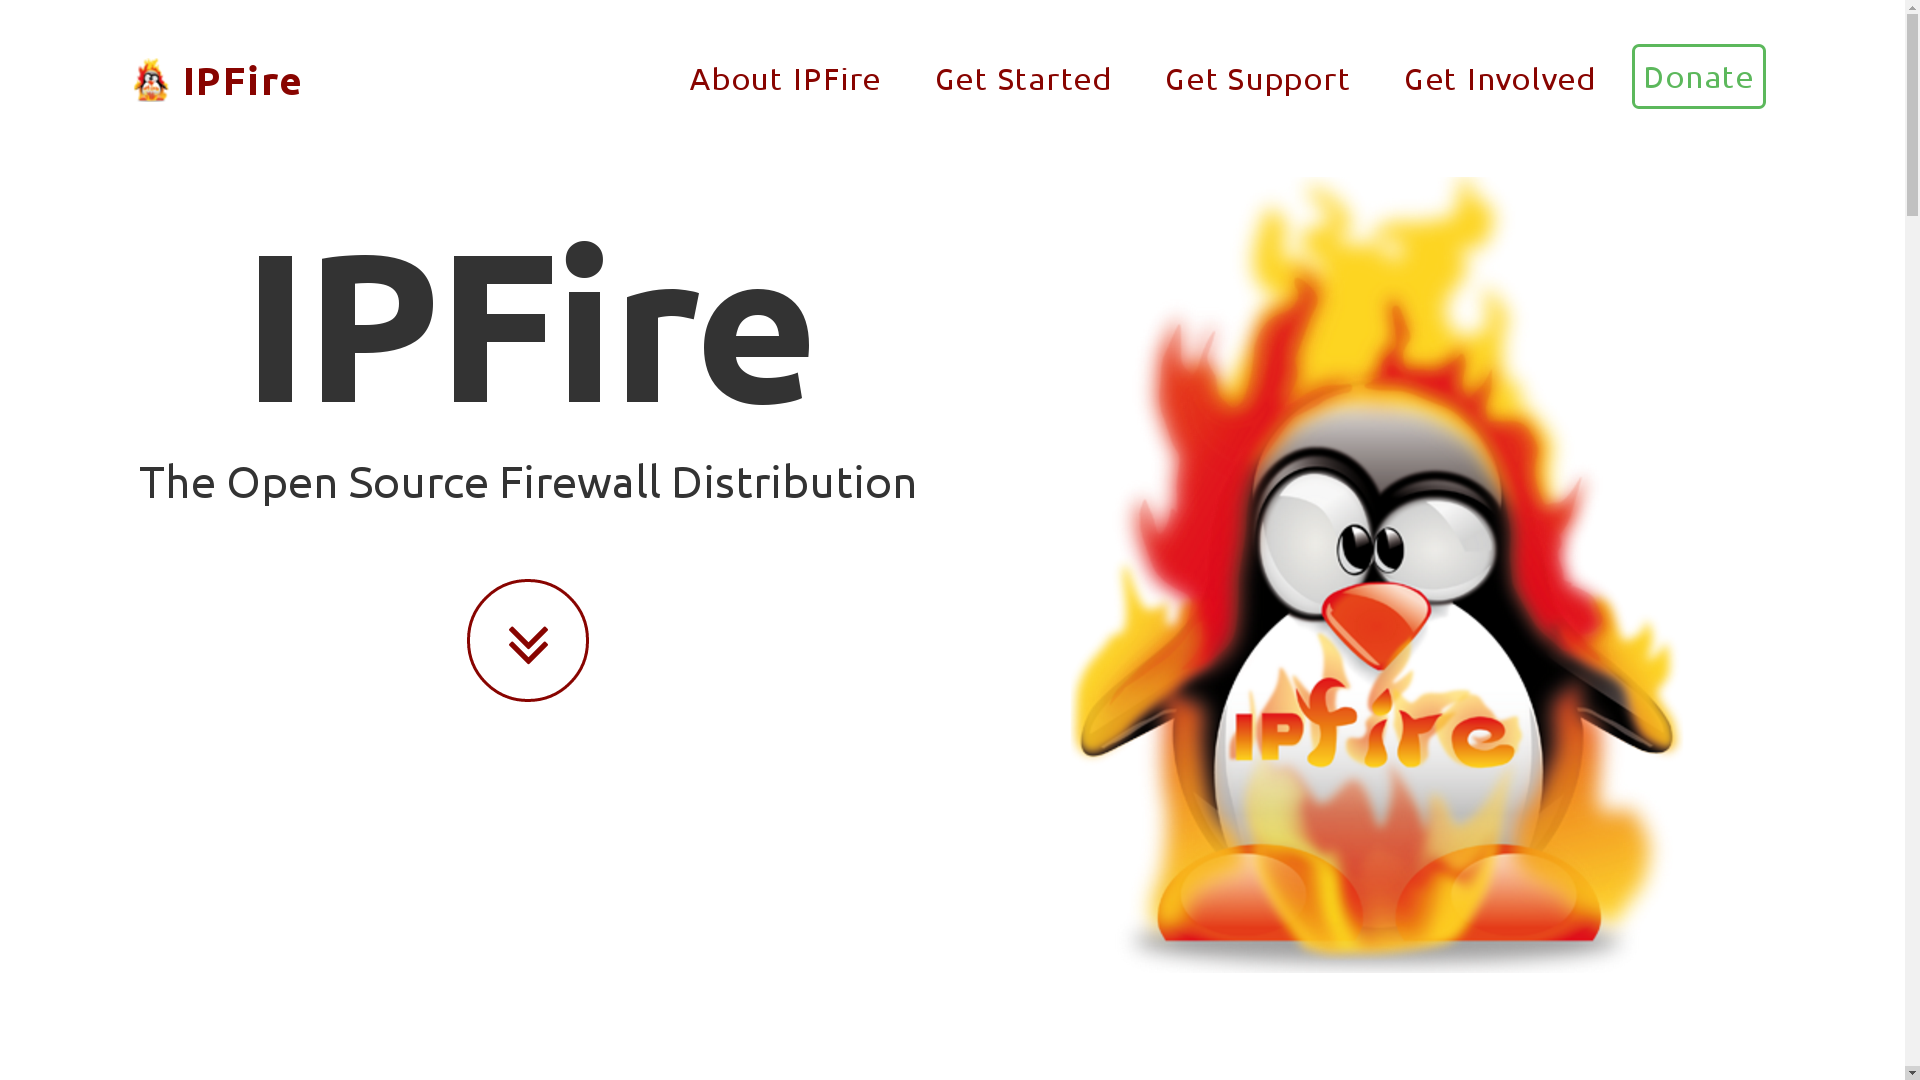
\includegraphics[keepaspectratio=true,height=1.10\textheight,width=1.00\textwidth,angle=0]{www-ipfire.png}
 \caption{IPFire Website}
 \label{fig:www-ipfire}
\end{figure}


\begin{itemize}
 \item Latest release: July 12th, 2016.
 \item \url{http://downloads.ipfire.org/releases/ipfire-2.x/2.19-core103/ipfire-2.19.x86_64-full-core103.iso}
 \item Installer has a cool thing that flashes the light on the ethernet port to identify it.
 \item Kernel: Linux 3.14.65-ipfire
 \item Post install, apache httpd process is starting, but not listening on any ports. Still in ``-k start''. So no web admin. Needed to modify listen.conf in Apache to 0.0.0.0:80 and 0.0.0.0:444. It appears it was hanging because of IPv6 (?).
 \item Nice MRTG-esque graphs of services and ports, including system temps, etc.
 \item Second set of non-MRTG network traffic graphs.
 \item Transparent web caching.
 \item Much more technical setup than clearOS. More SysAdmin oriented.
 \item OpenVPN.
 \item QoS.
 \item Load balancing? Fail over?
 \item IDS (snort).
 \item Uses its own pakfire package management tool.
 \item The wiki is under an NC license.
 \item Kernel uses grsec.
 \item No WAN failover (!).
\end{itemize}


\subsection{OPNsense}
 \href{https://opnsense.org/}{OPNsense} --- ``the Open Source Firewall that is easy-to-use and protects your network''

\begin{figure}[h!]
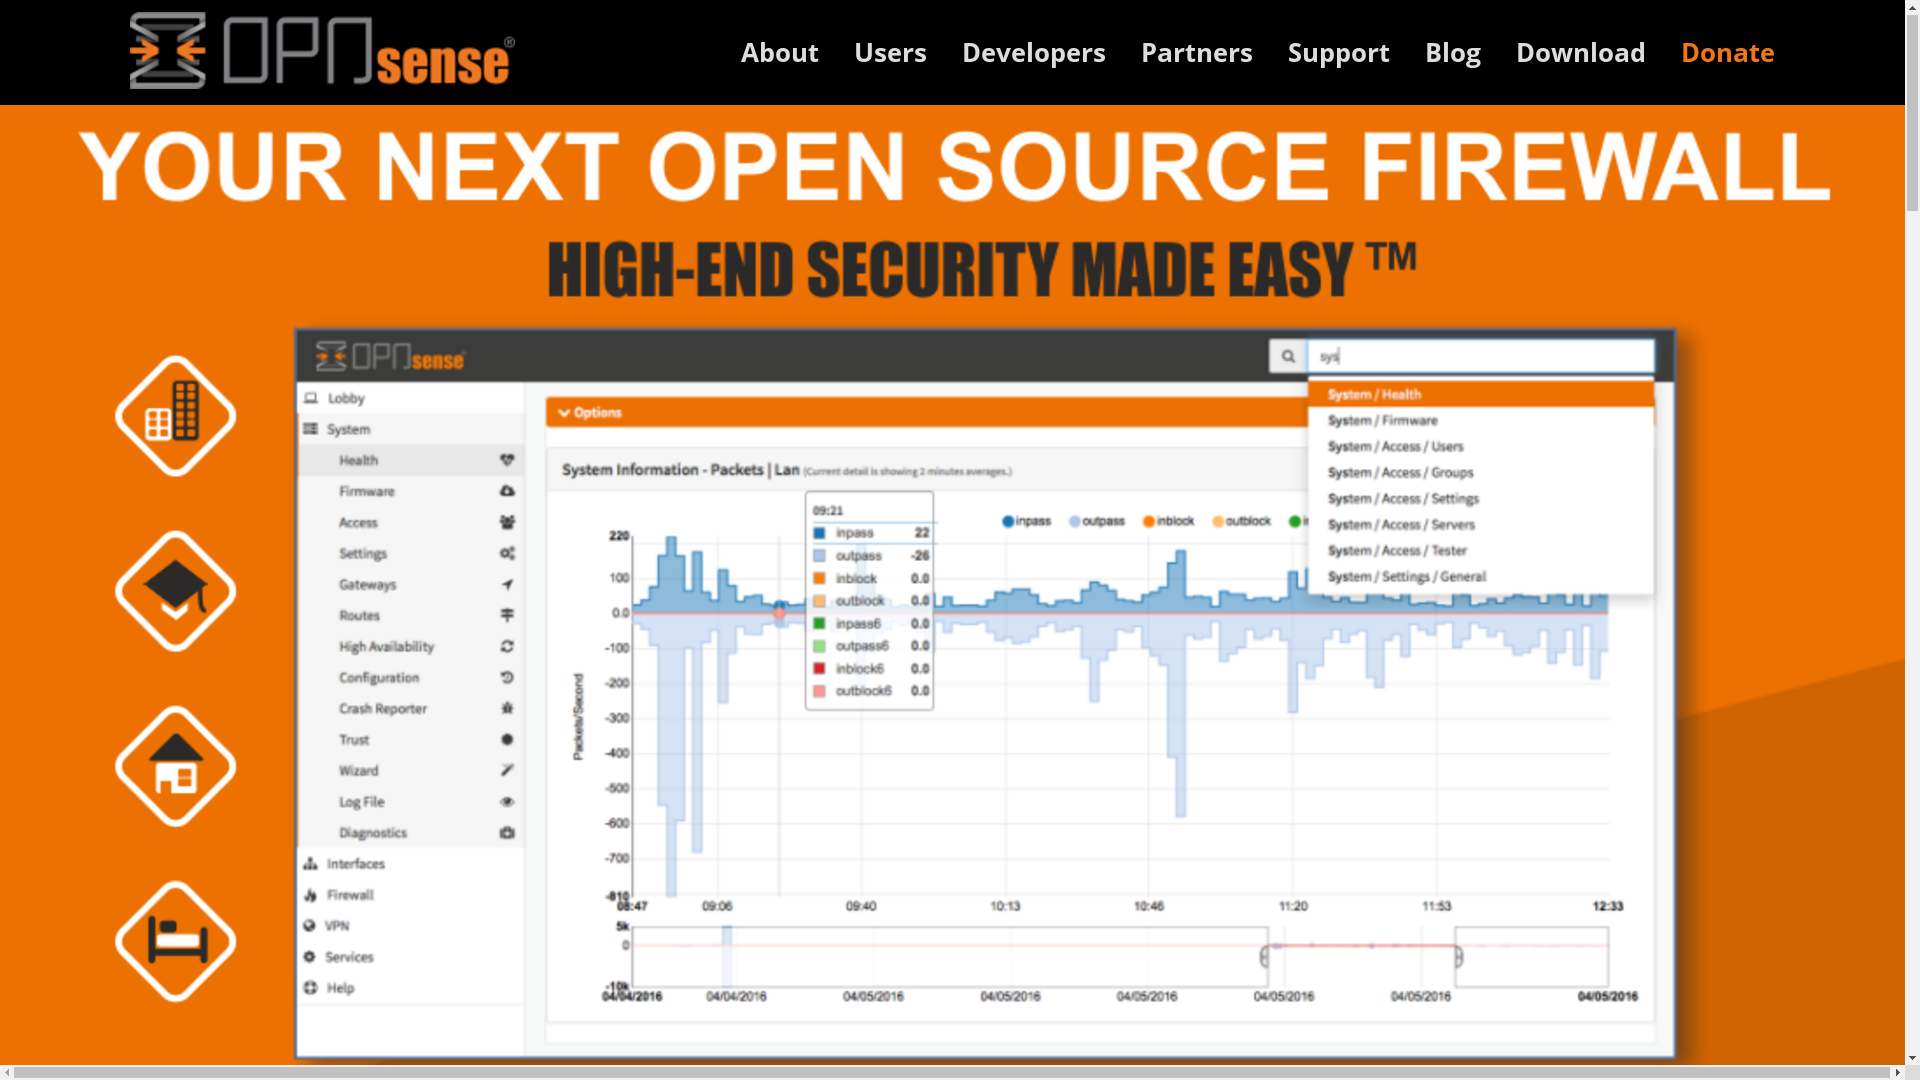
\includegraphics[keepaspectratio=true,height=1.10\textheight,width=1.00\textwidth,angle=0]{www-opnsense.png}
 \caption{OPNsense Website}
 \label{fig:www-opnsense}
\end{figure}

\begin{itemize}
 \item Release is current.
 \item Making a dd of the .iso to a USB drive didn't boot. OPNsense-16.7.r2-OpenSSL-cdrom-amd64.iso
 \item Based on FreeBSD.
 \item Source in github.
 \item Looks decent, but wasn't tested.
\end{itemize}


\section{Previous Operating Systems in Use}
\subsection{OpenBSD}
\href{https://www.openbsd.org/}{OpenBSD}

\begin{figure}[h!]
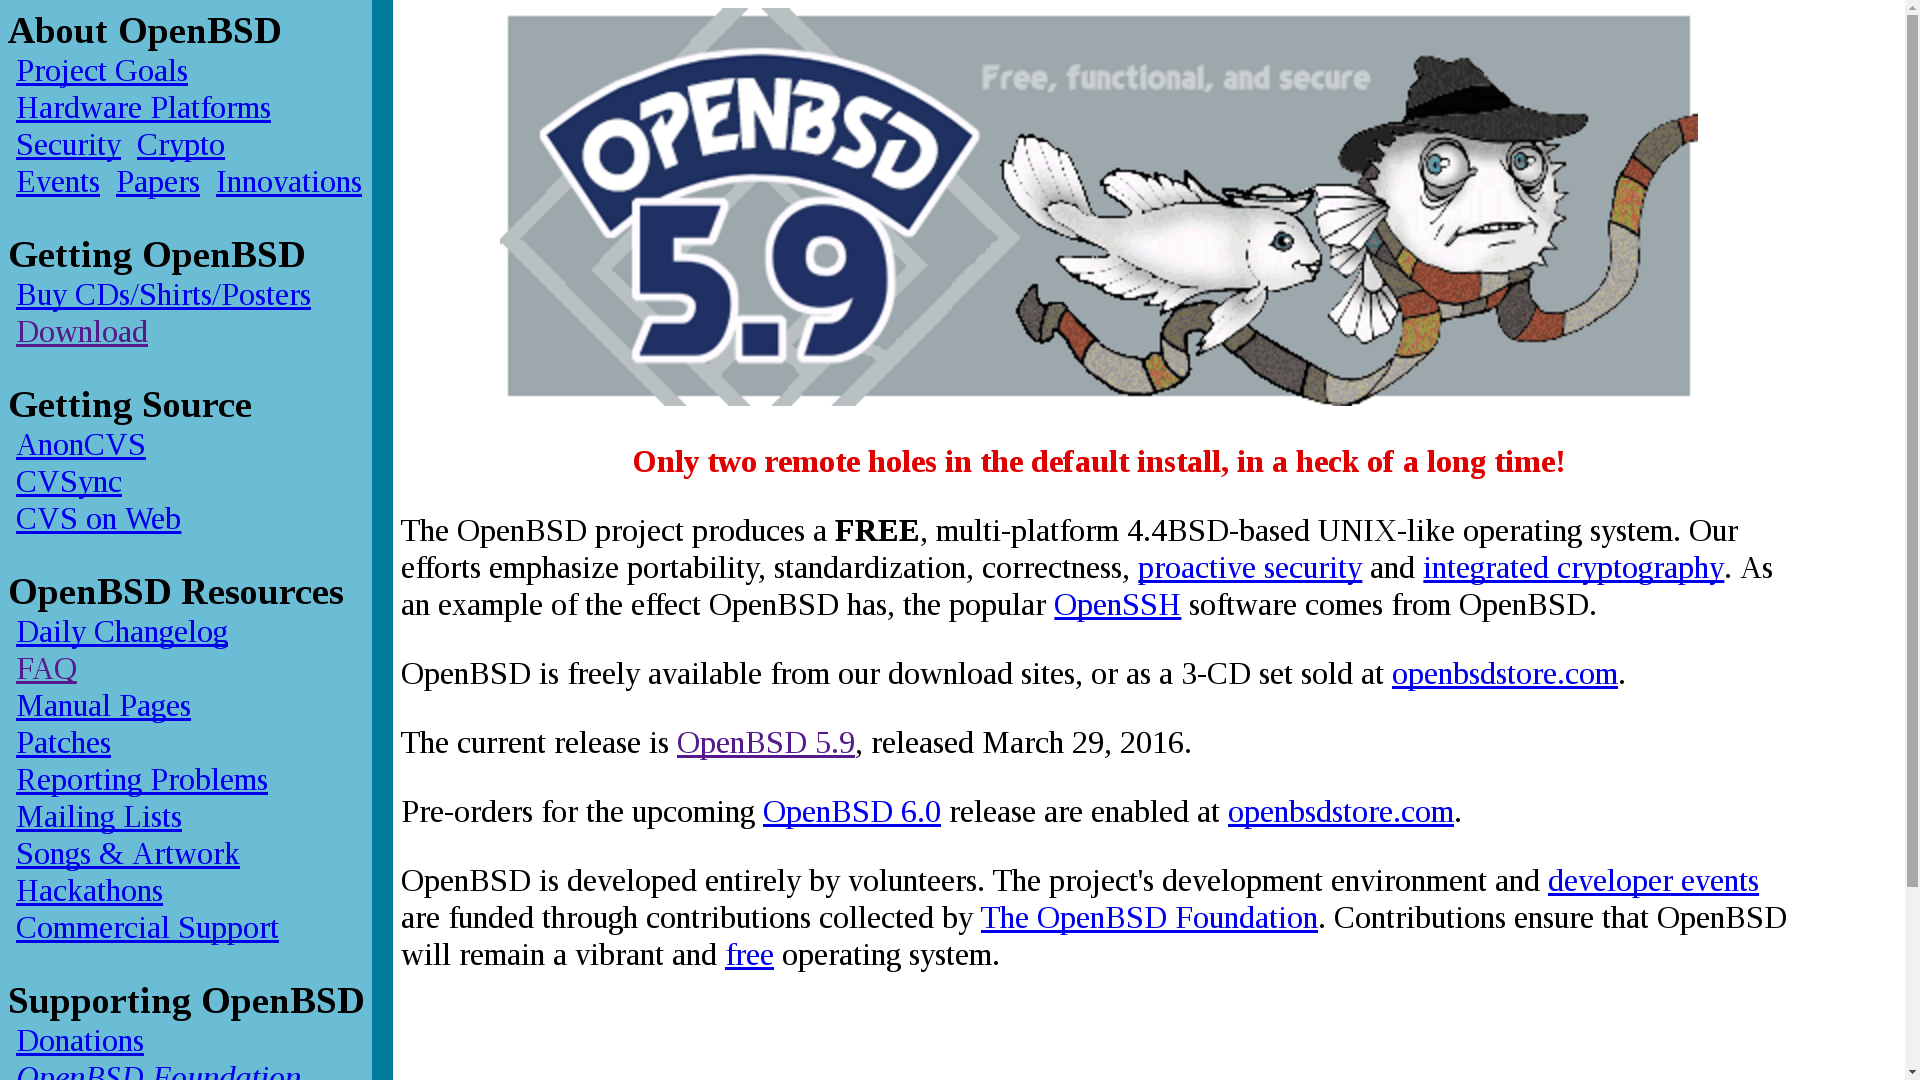
\includegraphics[keepaspectratio=true,height=1.10\textheight,width=1.00\textwidth,angle=0]{www-openbsd.png}
 \caption{OpenBSD Website}
 \label{fig:www-openbsd}
\end{figure}

Aleph Objects has dropped OpenBSD in favor of pfSense.

OpenBSD with PF was previously used for our firewall for the first five years.
It is very reliable and secure. Few people know how to administer it. It is
all command line editing of firewall configuration files.


\section{Other}
\subsection{Gentoo}
 \href{https://www.gentoo.org/}{Gentoo}

Can be tuned in.



\subsection{NetBSD}
 \href{https://www.netbsd.org/}{NetBSD}

Solid OS. Can use OpenBSD's pf, iirc. Same problem as with OpenBSD, few admins know it.


